% Include experiments here
Our experiments consisted of testing of 5 different training algorithms for RBMs. We use two variants of Contrastive Divergence  - Contrastive Divergence with one positive and negative phase (CD), and Persistent Contrastive Divergence (PCD). We used the three variants of PCD augmented with Parallel Tempering - vanilla Parallel Tempering (PT), Lifted Parallel Tempering (LPT) and Deterministic Even/Odd Algorithm (LPTD). 

\subsubsection{Experimental Setup}
We ran all of our experiments on a Norwegian Institute of Science and Technology Server, Beregningsserver - a 768 GB server with 28 Intel CPUs (2 $\times$ 14 Xeon 2.6 GHz cores).

We ran training on two different datasets. We used the Scikit-learn Digit Dataset, which consists of 1797 8 $\times$ 8 pixel images. In order to artificially increase the size of the dataset, we added translations of each image - shifted one pixel to up, one pixel down, one pixel to the left, and one pixel to the right. We also used the MNIST data set, consisting 60,000 28 $\times$ 28 pixel images. In order to speed up training, we used a subset of 10,000 images of the original MNIST dataset.

\subsubsection{Code Structure}
In order to implement our five algorithms, we augmented python's scikit-learn library \cite{pedregosa2011scikit}. All of our code is available at \url{https://github.com/Mittens2/532_proj}.

\subsection{Results}
For each experiment we tracked the evolution of the negative log likelihood as training progressed. We were focused on three main trends - the rate of convergence of the log likelihood, the maximum log likelihood achieved by each algorithm, and whether the log likelihood diverged after a certain amount of iterations.

\subsubsection{Scikit-Learn Digit Dataset}

We ran the five training variants for 100 passes of the full augmented Scikit-learn Digits Dataset with a batch size of 10, resulting in 71,880 weight updates for each algorithm. We optimized training over three hyperparameters - the number of hidden units $|h|$, the learning rate $\alpha$, and the batch size $n$. We used GridSearchCV with CD to select the hyperparameters to be used for training \cite{pedregosa2011scikit}. However, this just tended to select hyperparameters that resulted in the slowest training - i.e. the most hidden units available, with smallest batch size. Therefore, to speed up training, we reduced the number of hidden units, and increased $n$. The final setting of hyperparameters was chosen to be $|h|=50,  \alpha = 0.02$, and $n=10$.

\begin{figure}[ht!]
	\centering
	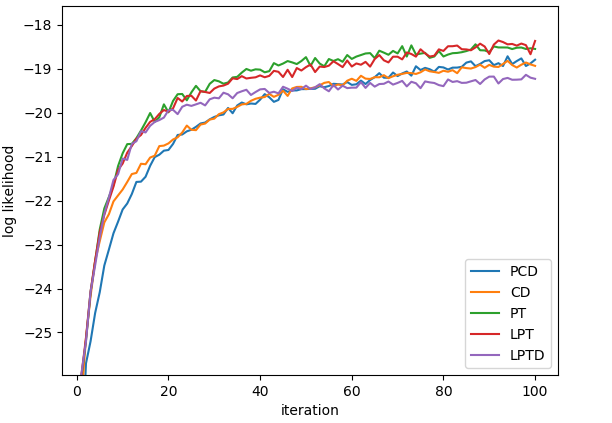
\includegraphics[scale=0.5]{digits.png}
\caption{Log Likelihood trend on Scikit-Learn Digits.}
\end{figure}

For the Parallel Tempering variants, we selected a temperature spacing, as well as number of chains to be run. We used a geometric temperature spacing such that $\beta_j = \gamma^j$  for $j = 0, ..., N$, which has been shown to work well in previous work \cite{kofke2002acceptance}. $\gamma$ and $N$ were optimized for vanilla PT resulting in $\gamma = 0.7$ and $N=6$.

The results obtained from plotting the negative log likelihood during training can be seen in Figure 2. In agreement with previous work on Parallel Tempering, it can be seen that the three variants of PT converge to a maximum log likelihood quicker than the two CD variants \cite{desjardins2010tempered}, \cite{fischer2014training}. Interestingly, the Deterministic Odd/Even Algorithm (LPTD), despite converging quickly, flatlines at a lower log likelihood than the other two variants, even being surpassed by the two CD variants as training goes on. No difference is observed in the efficacy of PT and LPT. The inferior performance of LPTD can be attributed to the excessive emphasis on exploring low probability regions in the sample space. The Scikit-learn Digits Dataset is a fairly simple dataset, with the modes of the data being fairly close together, and thus there is not a significant advantage in having a highly exploratory algorithm.

In order to test this hypothesis, we ran our five variants on the MNIST dataset, which consists of much higher resolution digit images, resulting in farther modes in the sample space.

\subsubsection{MNIST Dataset}
We ran each variant for 50 passes of a subset of the MNIST dataset with a batch size of 100, resulting in 5,000 weight updates per training algorithm. In conjunction with previous research on RBM training with PT, we used 500 hidden units, with a learning rate of 0.01\cite{desjardins2010tempered}. 

\begin{figure}[ht!]
	\centering
	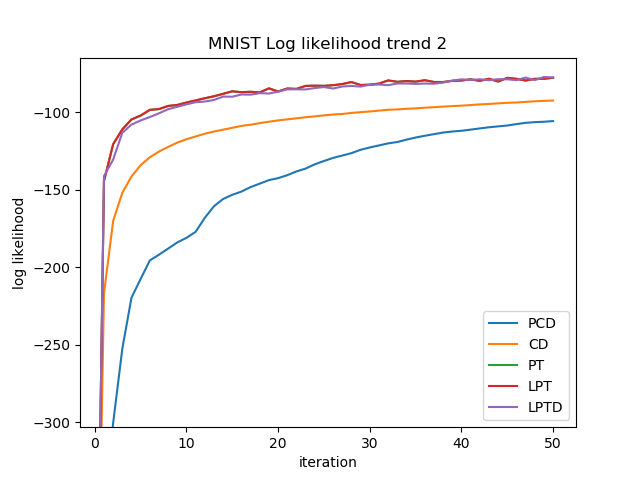
\includegraphics[scale=0.25]{MNIST.png}
\caption{Log Likelihood trend on MNIST.}
\end{figure}

We used the same PT hyperparameters as were used in the previous experiment - $\gamma_0 = 0.7$ with $N=6$. The trend of the negative log likelihood as training progressed is plotted in Figure 2. As can be seen, once again the three variants of PT converge to a max log likelihood quicker than the two CD variants. As hypothesized, LPTD does better on data with more sparse modes. However, no PT variant performs better than another, suggesting that the added exploratory behaviour of LPT and LPTD is not enough to make a significant difference when learning data.  

\section{Discussion}
In this study we describe the results obtained by using 5 different algorithms for training RBMs. Our results support previous results on RBM training with PT, showing that augmenting PCD with multiple parallel temperature chains results in a significant increase the speed of convergence for training. Our results also show that allocating more computational power to increase the exploratory behaviour of PT, i.e. using Lifted Parallel Tempering, or using the Deterministic Even/Odd algorithm does not make training more effective, at least on the datasets that were considered for this study.

More computational power is required in order to use PT variants during RBM training. However, since the augmentation can be run mostly in parallel, when there are many computing resources available, then it is advantageous to run PCT with PT. At least for now, using more advanced versions of PT for RBM training does not seem promising. Interestingly, the Even/Odd algorithm is often chosen when implementing PT for RBMs, due to its highly parallel structure \cite{fischer2014training}. However, our results show that this might not be optimal, especially when the modes in the sample space are close together.

More research needs to be done in order to fully assess the power of these more complex Parallel Tempering methods. Perhaps with a more complex dataset, LPT and LPTD will result in more efficient training of the models. \\